\chapter{Implementacija i korisničko sučelje}
		
		
		\section{Korištene tehnologije i alati}
		
		
			Komunikacija unutar tima odvijala se putem aplikacija \underline{WhatsApp}\footnote {\url{https://www.whatsapp.com/}} i \underline{Discord} \footnote{\url{https://discord.com}}, a s profesorom smo komunicirali putem \underline{MS Teamsa} \footnote{\url{https://www.microsoft.com/hr-hr/microsoft-teams/group-chat-software/}}.
			
			
			Za izradu UML dijagrama korišten je alat \underline{Astah Professional} \footnote {\url{https://astah.net/downloads/}} (studentska licenca), a za izradu ER dijagrama javno dostupan alat \underline{dbdiagram} \footnote {\url{https://dbdiagram.io/home}}.
			
			Verzioniranje koda olakšale su nam platforme \underline{Git} \footnote {\url{https://git-scm.com/}}  i \underline{GitLab} \footnote {\url{https://gitlab.com/}}  na kojem je dostupan udaljeni repozitorij s kojeg i na koji članovi razvojnog tima mogu preuzimati/postavljati kod i projektnu dokumentaciju.
			
			 Dokumentacija je pisana unutar okoline \underline{TeXstudio} \footnote {\url{https://www.latex-project.org/}} koja olakšava pisanje u \underline{LaTeX-u} \footnote {\url{https://www.texstudio.org/}} koji omogućuje izradu strukturiranog i preglednog dokumenta.
			
		
			Članovi tima su koristili razvojno okruženje s kojim su od ranije upoznati, \underline{Microsoft Visual Studio } \footnote {\url{https://visualstudio.microsoft.com/}}. Integrirana razvojna okruženja (\textit{engl. integrated development environment (IDE)}) programerima pružaju grafičko sučelje za pisanje koda u različitim programskih jezicima, usporedni pregled različitih projekata i druge pogodnosti poput uočljivog formatiranja koda i olakšanog otkrivanja i ispravljanja pogrešaka. 
			
			Osim ručnog testiranja aplikaciju smo testirali pomoću radnog okvira \underline{Selenium} \footnote {\url{https://www.selenium.dev/}}. Važno je biti svjestan da je nepostojanje pogreške, bez formalne verifikacije, nemoguće utvrditi.
			
			Poslužiteljska strana aplikacije implementirana je koristeći radni okvir za razvoj web aplikacija \underline{Django } \footnote {\url{https://www.djangoproject.com/}}(jezik \underline{Python 3.8} \footnote {\url{https://www.python.org/downloads/}}). Prednosti uporabe ovog (i sličnih) radnih okvira su olakšana implementacija čestih funkcionalnosti, komunikacija s bazom podataka, osigurana određena razina sigurnosti i općenito olakšana izgradnja programske potpore. Za bazu podataka odabrana je baza \underline{PostgreSQL }\footnote {\url{https://www.postgresql.org/}},  na glasu kao pouzdana i robusna relacijska baza podataka.
			Za izradu klijentske strane tradicionalno je korišten \underline{HTML}\footnote {\url{https://developer.mozilla.org/en-US/docs/Web/HTML}}, \underline{CSS}\footnote {\url{https://www.w3.org/Style/CSS/Overview.en.html}} i \underline{JavaScript} \footnote {\url{	https://www.javascript.com/}}. Izradu korisničnog sučelja olakšao nam je razvojni okvir \underline{Bootstrap}\footnote {\url{https://getbootstrap.com/}} s mnoštvom javno dostupnih stilova za često korištene HTML elemente. Pri dizajniranju izgleda stranice korištene su i SVG ikonice javno dostupne na stranici \underline{FreeSVG} \footnote {\url{https://freesvg.org/}}. 
		
			Radi pouzdanosti i neovisnosti aplikacije obavljena je virtualizacija korištenjem platforme\underline{ Docker} \footnote {\url{https://www.docker.com/}}, a objavljena je na javnom poslužitelju pomoću \underline{Digital Oceana} \footnote {\url{https://www.digitalocean.com/}}, brzorastuće platforme zasnovane na računarstvu u oblaku (\textit{engl. cloud computing}), koja između ostalih pruža uslugu objave aplikacija (\textit{engl. cloud hosting}). Na poslužitelju, tzv. \textit {dropletu}, konfigurirali smo dva kontejnera, jedan za aplikaciju i jedan za bazu podataka. \newline

		
			
			Temeljna je svrha svih navedenih tehnologija i alata ubrzati i pojednostaviti razvoj programske potpore visoke kvalitete.
					
			\eject 
		
	
		\section{Ispitivanje programskog rješenja}
			
			\textbf{\textit{dio 2. revizije}}\\
			
			 \textit{U ovom poglavlju je potrebno opisati provedbu ispitivanja implementiranih funkcionalnosti na razini komponenti i na razini cijelog sustava s prikazom odabranih ispitnih slučajeva. Studenti trebaju ispitati temeljnu funkcionalnost i rubne uvjete.}
	
			
			\subsection{Ispitivanje komponenti}
			\textit{Potrebno je provesti ispitivanje jedinica (engl. unit testing) nad razredima koji implementiraju temeljne funkcionalnosti. Razraditi \textbf{minimalno 6 ispitnih slučajeva} u kojima će se ispitati redovni slučajevi, rubni uvjeti te izazivanje pogreške (engl. exception throwing). Poželjno je stvoriti i ispitni slučaj koji koristi funkcionalnosti koje nisu implementirane. Potrebno je priložiti izvorni kôd svih ispitnih slučajeva te prikaz rezultata izvođenja ispita u razvojnom okruženju (prolaz/pad ispita). }
			
			 
			\noindent  \textbf{Ispitni slučaj 1: Dodavanje administratora}\\
			 \textbf{Ulaz:}
			 \begin{packed_enum}
			 	\item {Prijava u sustav kao administrator}
			 	\item {Ulaz u administracijsko sučelje klikom na gumb u izbornoj traci}
			 	\item {Unos neispravnih korisničkih podataka novog administratora}
			 	\item {Unos ispravnih korisničkih podataka novog administratora}
			 \end{packed_enum}
			 
			 \textbf{Očekivani rezultat:}
			 \begin{packed_enum}
			 	\item {Uspješna prijava u sustav}
			 	\item {Otvaranje administracijskog sučelja}
			 	\item {Dojava greške o neispravnoj adresi e-pošte}
			 	\item {Potvrda o dostavi korisničkih podataka novog administratora na adresu e-pošte}
			 \end{packed_enum}
			 \textbf{Rezultat: }Prijava u postojeći administratorski račun je uspješna, unos neispravne adrese e-pošte pri unosu podataka novog administratora ispravno dojavljuje grešku, a prilikom unosa ispravnih korisničkih podataka ispravno se prikazuje potvrda o dostavljenim podatcima na adresu e-pošte. {\color{green} Aplikacija prolazi test.}\\
			
			 \noindent \textbf{Ispitni slučaj 2: Dodavanje novih sekcija}\\
			 \textbf{Ulaz:}
			 \begin{packed_enum}
			 	\item {Prijava u sustav kao administrator}
			 	\item {Ulaz u administracijsko sučelje klikom na gumb u izbornoj traci}
			 	\item {Unos već postojeće sekcije}
			 	\item {Unos nove sekcije}
			 \end{packed_enum}
			 \textbf{Očekivani rezultat:}
			 \begin{packed_enum}
			 	\item {Uspješna prijava u sustav}
			 	\item {Otvaranje administracijskog sučelja}
			 	\item {Dojava greške o već postojećoj sekciji}
			 	\item {Nova sekcija dodanu u listu sekcija}
			 \end{packed_enum}
			 \textbf{Rezultat: }Prijava u postojeći administratorski račun je uspješna i otvara se administracijsko sučelje. Pokušaj dodavanja sekcije koja već postoji ispravno javlja pogrešku o pokušaju unosa već postojeće sekcije. Unos nove sekcije je uspješan i ispravno se dodaje na listu sekcija. {\color{green} Aplikacija prolazi test.}\\
			
			
			 \noindent \textbf{Ispitni slučaj 3: Registracija kao recenzent}\\
			  \textbf{Ulaz:}
			 \begin{packed_enum}
			 	\item {Klik na gumb za registraciju u izbornoj traci}
			 	\item {Unos podataka za registraciju}
			 	\item {Odabir registracije kao recenzent}
			 \end{packed_enum}
			 \textbf{Očekivani rezultat:}
			 \begin{packed_enum}
			 	\item {Otvara se sučelje za registraciju}
			 	\item {Odabirom registracije kao recenzent mijenjaju se polja obrasca prijave}
			 	\item {Obavijest o potrebi da predsjedavajući potvrdi registraciju}
			 \end{packed_enum}
			  \textbf{Rezultat: }Sučelje za registraciju otvara se nakon klika na gumb registracije. Nakon sto se označi gumb da se korisnik prijavljuje kao recenzent, obrazac prijave se mijenja i traži se odabir sekcije za koju se korisnik registrira. Po završetku prijave ispravno se javlja obavijest kako je potrebno da predsjedavajući potvrdi registraciju prije mogućnosti recenziranja. {\color{green} Aplikacija prolazi test.}\\
			
			
			 \noindent \textbf{Ispitni slučaj 4: Potvrda prijave recenzenta od predsjedavajućeg}\\
			  \textbf{Ulaz:}
			 \begin{packed_enum}
			 	\item {Prijava u sustav kao predsjedavajući}
			 	\item {Otvaranje upravljačkog sučelja}
			 	\item {Klik na gumb "Potvrdi"}
			 \end{packed_enum}
			  \textbf{Očekivani rezultat:}
			 \begin{packed_enum}
			 	\item {Izborna traka se mijenja i pojavljuje se gumb za otvaranje upravljačkog sučelja predsjedavajućeg}
			 	\item {Otvara se upravljačko sučelje predsjedavajućeg}
			 	\item {Prijava se prihvaća i recenzentu šalje se e-pošta s podacima za prijavu}
			 \end{packed_enum}
			 \textbf{Rezultat: }Prijavom kao predsjedavajući mijenja se izborna traka i pojavljuje se gumb za otvaranje upravljačkog sučelja predsjedavajućeg konferencije. Otvaranjem sučelja vidljiv je popis recenzenata koji čekaju potvrdu registracije. Klikom na gumb "Potvrdi" recenzentu se šalje e-pošta s potrebnim podacima za prijavu. {\color{green} Aplikacija prolazi test.}\\
			\eject 

		\subsection{Ispitivanje sustava}
			
			Za testiranje sustava odabran je radni okvir Selenium IDE\footnote{\url{https://www.selenium.dev/selenium-ide/}} radi njegove jednostavnosti korištenja te sličnosti ponašanju stvarnog korisnika. Odabrani testovi usredotočeni su na administrativne zadatke sustava i pokrivaju velik broj obrazaca uporabe.\\ 
		
		
		\section{Dijagram razmještaja}
			 
			 
			\begin{figure}[H]
			 	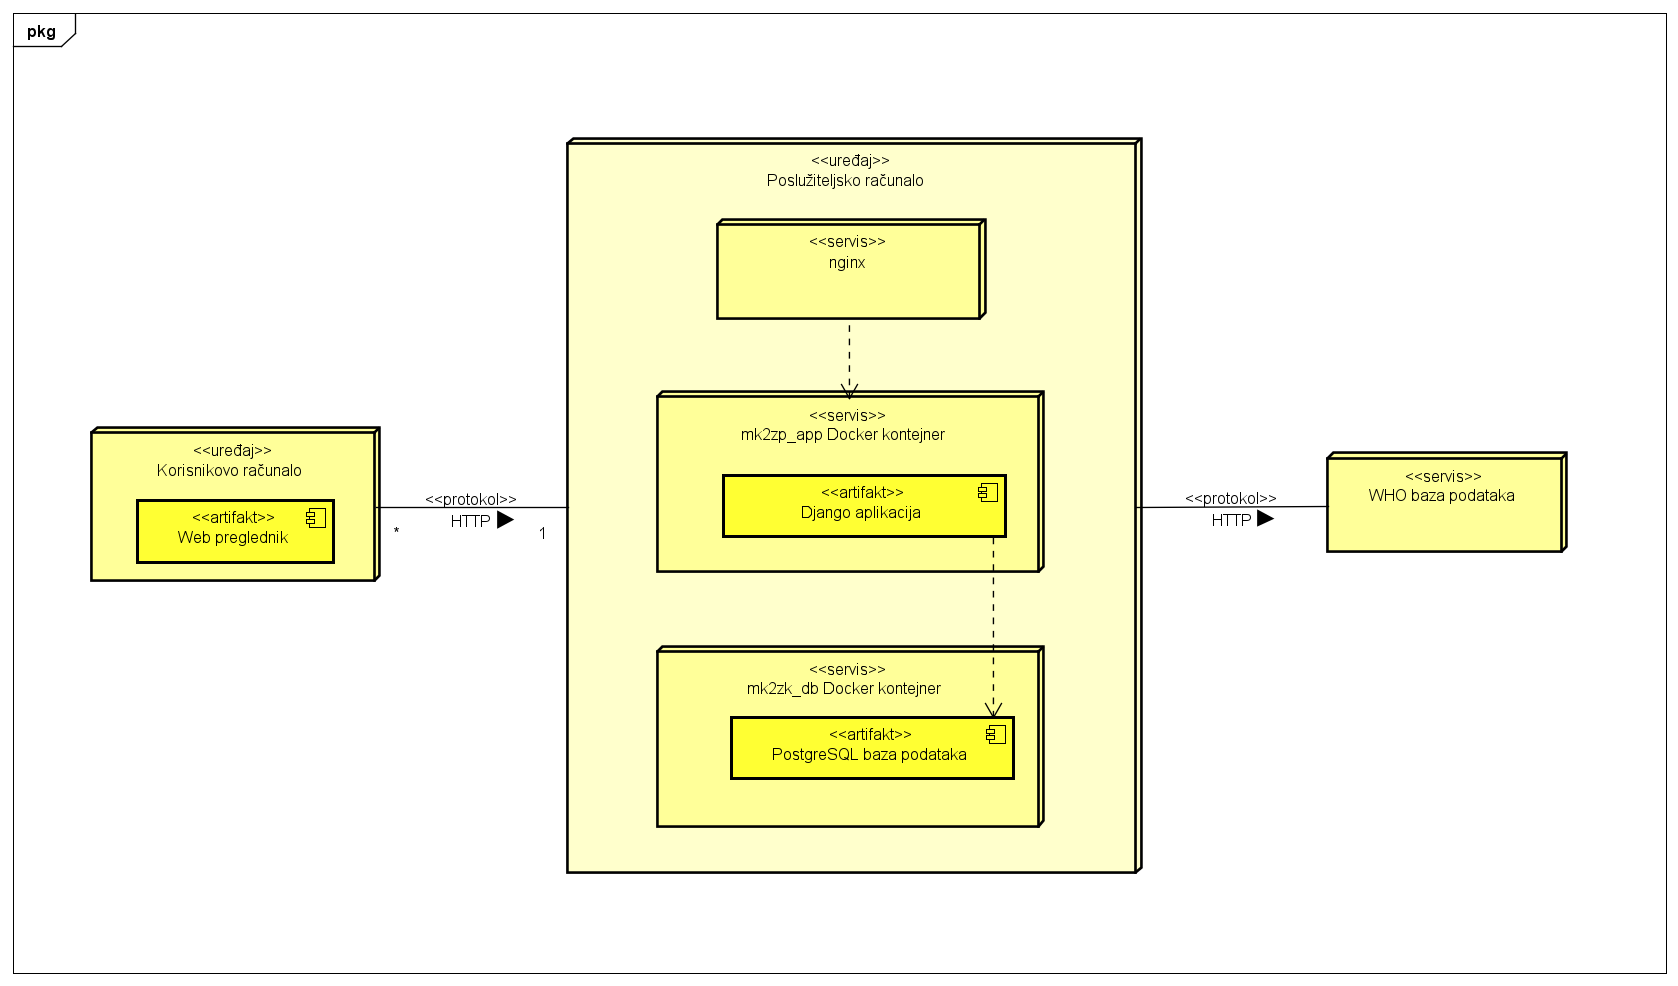
\includegraphics[width= 15 cm, height= 25 cm, keepaspectratio]{dijagrami/Diagram razmjestaja.png} 
			 	\centering
			 	\caption{Dijagram razmještaja - Znanstvena konferencija}
			 	\label{fig:act5}
			 \end{figure}
			
			\eject 
		
		\section{Upute za puštanje u pogon}
		
			\textbf{\textit{dio 2. revizije}}\\
		
			 \textit{U ovom poglavlju potrebno je dati upute za puštanje u pogon (engl. deployment) ostvarene aplikacije. Na primjer, za web aplikacije, opisati postupak kojim se od izvornog kôda dolazi do potpuno postavljene baze podataka i poslužitelja koji odgovara na upite korisnika. Za mobilnu aplikaciju, postupak kojim se aplikacija izgradi, te postavi na neku od trgovina. Za stolnu (engl. desktop) aplikaciju, postupak kojim se aplikacija instalira na računalo. Ukoliko mobilne i stolne aplikacije komuniciraju s poslužiteljem i/ili bazom podataka, opisati i postupak njihovog postavljanja. Pri izradi uputa preporučuje se \textbf{naglasiti korake instalacije uporabom natuknica} te koristiti što je više moguće \textbf{slike ekrana} (engl. screenshots) kako bi upute bile jasne i jednostavne za slijediti.}
			
			
			 \textit{Dovršenu aplikaciju potrebno je pokrenuti na javno dostupnom poslužitelju. Studentima se preporuča korištenje neke od sljedećih besplatnih usluga: \href{https://aws.amazon.com/}{Amazon AWS}, \href{https://azure.microsoft.com/en-us/}{Microsoft Azure} ili \href{https://www.heroku.com/}{Heroku}. Mobilne aplikacije trebaju biti objavljene na F-Droid, Google Play ili Amazon App trgovini.}
			
			
			\eject 